\begin{introduction}
    \item 经典谐振子
\end{introduction}

\section{经典谐振子}
经典谐振子的运动模式遵循Hooke定律,即满足:
\begin{equation}
    F=-kx
\end{equation}

其中$F$称为回复力,$k$称为弹簧的弹性系数。我们对Hooke定律运用Newton第二定律,即可得到经典谐振子的运动方程:
\begin{equation}
    \frac{d^2x}{dt^2}+\omega^2x=0
\end{equation}

其中$\omega=\sqrt{\frac{k}{m}}$,称为弹簧的角频率,是描述弹簧本身性质的物理量。求解这个方程,我们可以得到位移随时间的变换关系,也就是方程的通解:
\begin{equation}
    x(t)=A\cos{\omega t}+B\sin{\omega t}
\end{equation}

其中系数A和B可以根据初始条件求得。进一步,我们可以求出弹簧的势能为:
\begin{equation}
    V(x)=\frac{1}{2}kx^2
\end{equation}

当然上述两式只能描述简谐振动的情况,因为不仅要忽略外力的作用,而且当弹簧拉伸接近或者超过弹性系数的时候,Hooke定律都是不适用的,但是当势能取极小值的时候,我们还是能够用简谐振动近似极小点附近运动的情况的(如\ref{fig:HookeLaw}):
\begin{figure}[H]
    \centering
    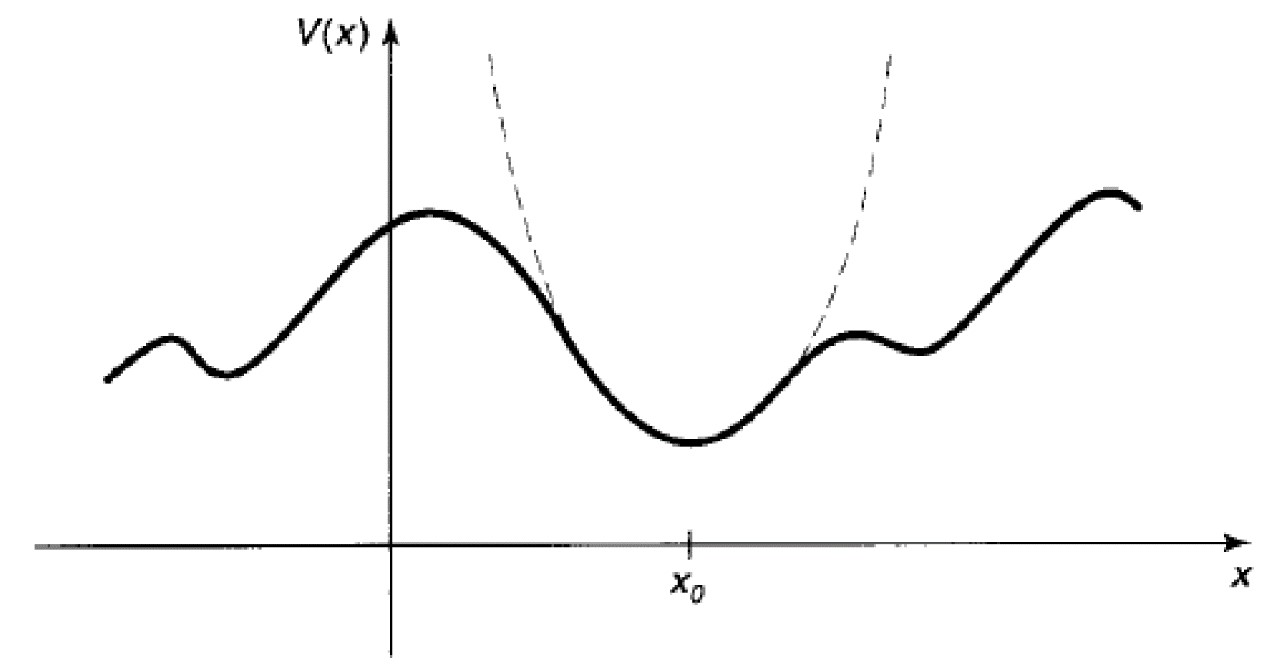
\includegraphics[width=0.9\textwidth]{figure/HookeLaw.jpg}
    \caption{简谐振动能够近似极小点附近的运动情况}
    \label{fig:HookeLaw}
\end{figure}

具体来说,我们可以对势能函数的极小点作Taylor展开:
\begin{equation}
    V(x)=V(x_0)+V'(x_0)(x-x_0)+\frac{1}{2}V''(x_0)(x-x_0)^2+\dots
\end{equation}

由于$x_0$是极小点,因此我们可以人为地令$x=x_0$处于势能零点,因此$V(x_0)=0$。同时,由于极小点的性质,$V'(x_0)=0$,所以势能函数在忽略高阶无穷小量时可以写成:
\begin{equation}
    V(x)\cong \frac{1}{2}V''(x_0)(x-x_0)
\end{equation}

这正是描述简谐运动的势能,其有效弹性系数为$k=V''(x_0)$。虽然简谐运动是简化的模型,但是其在实际情况中的实用性使得研究简谐振动是非常有必要的。